\section{Razsevni diagram in vzorčni koeficient korelacije}\label{sec3}

Prikažimo dobljene podatke na razsevnem diagramu:

\begin{figure}[h]
    \centering
    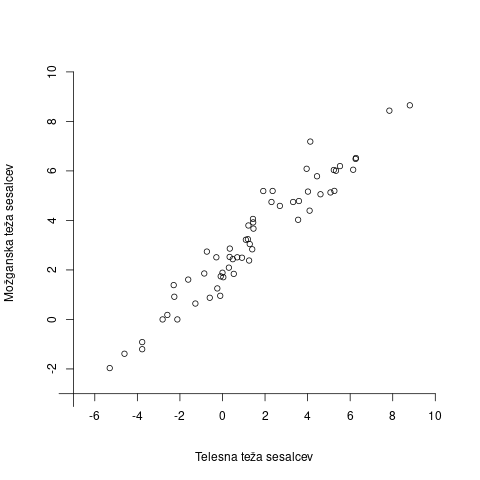
\includegraphics[scale=0.5]{res/razsevni-diagram.png}
    \caption{Razsevni diagram telesne in možganske teže sesalcev}
    \label{img:razs-diag}
\end{figure}

\noindent
Za izris grafa smo uporabili naslednjo R kodo:

\begin{verbatim}
    plot(
        x = log(mozgani$telteza),
        y = log(mozgani$mozteza),
        xlab = "Telesna teža sesalcev",
        ylab = "Možganska teža sesalcev",
        xlim = c(-7, 10),
        ylim = c(-3, 10),
        axes = FALSE
    )

    axis(1, pos = -3, at = seq(-8, 10, by = 2))
    axis(2, pos = -7, at = seq(-4, 10, by = 2))
\end{verbatim}

\newpage
Funkcija \verb|plot()| nam izriše razsevni diagram s podanimi parametri, v našem primeru z naslednjimi parametri:

\begin{itemize}
    \item \verb|x = log(mozgani$telteza)|, kjer \verb|x| predstavlja logaritemsko funkcijo telesne teže sesalcev,
    \item \verb|y = log(mozgani$mozteza)|, kjer \verb|y| predstavlja logaritemsko funkcijo možganske teže sesalcev,
    \item \verb|xlab| in \verb|ylab|, ki predstavljata ime x in y osi,
    \item \verb|xlim| in \verb|ylim|, ki določita začetne in končne koordinate x in y osi in
    \item \verb|axes = FALSE|, ki odstrani privzete koordinatne osi, saj jih želimo zamenjati z osmi, primernimi za
    naše parametre.
\end{itemize}

\noindent
Za izris koordinatnih osi uporabimo funkcijo \verb|axis()| s parametri \emph{1} ali \emph{2}, ki predstavljata
y in x os, \emph{pos}, ki predstavlja pozicijo postavitve osi, in \verb|at = seq()|, ki določi oznake na oseh
(s parametri \verb|seq(začetek, konec, razmak)|).
Moč korelacije lahko preverimo s \emph{Pearsonovim koeficientom}, kar v R naredimo z ukazom

\noindent
\verb|(r = cor(mozgani$telteza, mozgani$mozteza))|\label{en:r}, ki nam vrne rezultat \verb|[1] 0.9340911|.
Vrednost vzorčnega koeficienta korelacije je zelo visoka (r = 0.934), kar nakazuje visoko linearno povezanost
telesne teže sesalcev in teže njihovih možganov.
Ker je koeficient pozitiven nam to pove, da se z večjo telesno težo sesalca veča tudi teža njegovih možganov.